\subsection{Pila de arena de Bak–Tang–Wiesenfeld}\label{sec:exp1_sandpile}

El siguiente experimento tiene el objetivo de replicar el comportamiento del sistema autoorganizado llamado \textit{sandpile}. Como se menciono anteriormente, es un sistema bidimensional que agrega granos de arena a una celula que, cuando alcanza un umbral, pierde sus granos y los distribuye en en sus vecinos.

En un sentido estricto, el modelo de \textit{sandpile} no es un automata celular, porque el sistema recibe constantemente una entrada (el grano de arena en el centro) que depende de la salida del sistema (cuando esta en equilibrio). 

Para representar este sistema mediante un autómata celular se agrega un nuevo subconjunto de estados que representan el flujo constante de arena en cada paso evolutivo. 

Sea el conjunto $\mathcal{S}_b = \{0,1,2,3,4, 5, 6, 7\}$ los estados que definen la altura y sea $\mathcal{S}_i = \{ 0_i, 1_i, 2_i, 3_i, 4_i, 5_i, 6_i, 7_i, 8_i\}$ los estados que definen la altura y que añaden granos, definimos entonces $\mathcal{S} = \mathcal{S}_b \cup \mathcal{S}_i$ como el conjunto completo de estados. 

Aunque el umbral de disperción esta definido por cuatro estados, se definen siete alturas para incluir todos los escenarios posibles. Por ejemplo: 
\[
\left[\begin{matrix}
	0 & 4 & 0 \\
	4 & 3 & 4 \\
	0 & 4 & 0
\end{matrix}\right] \rightarrow
\left[\begin{matrix}
	2 & 0 & 2 \\
	0 & 7 & 0 \\
	2 & 0 & 2
\end{matrix}\right] \rightarrow
\left[\begin{matrix}
	2 & 1 & 2 \\
	1 & 3 & 1 \\
	2 & 1 & 2
\end{matrix}\right]
\]
Del mismo modo, los estados generadores incluyen un estado adicional. Derivado del ejemplo anterior, si una célula generadora recibe su máximo, adicionalmente en el siguiente paso recibe un grano adicional, lo que causa una nueva dispersión:
\[
\left[\begin{matrix}
	0 & 4 & 0 \\
	4 & 3_i & 4 \\
	0 & 4 & 0
\end{matrix}\right] \rightarrow
\left[\begin{matrix}
	2 & 0 & 2 \\
	0 & 8_i & 0 \\
	2 & 0 & 2
\end{matrix}\right] \rightarrow
\left[\begin{matrix}
	2 & 1 & 2 \\
	1 & 5_i & 1 \\
	2 & 1 & 2
\end{matrix}\right] \rightarrow
\left[\begin{matrix}
	2 & 2 & 2 \\
	2 & 2_i & 2 \\
	2 & 2 & 2
\end{matrix}\right]
\]

Existen $|\mathcal{S}| = 17$ estados y una vecindad Von Neumman (5 vecinos). El vector de regla tiene un tamaño de $17^5 = 1419857$, y la regla del autómata celular que replica \textit{sandpile} es una entre $17^1419857$ posibles reglas. Su orden de complejidad es mucho mayor comparado con B3/S23. Es por esto que el objetivo de autómata celular neuronal sera descifrar la regla que imite este comportamiento.

Con esta definición propuesta, fueron generadas 100 condiciones aleatorias con cuatro generadores en un espacio de $50 \times 50$ durante 1500 pasos. 

De acuerdo con la figura \ref{fig:sp_proportion} existen estados, como $8_i$ que tiene una probabilidad de aparición muy baja. Sin embargo, esta probabilidad esta determinada por que las pruebas solo consideran cuatro de 2500 células. 

\begin{figure}[H]
	\centering
	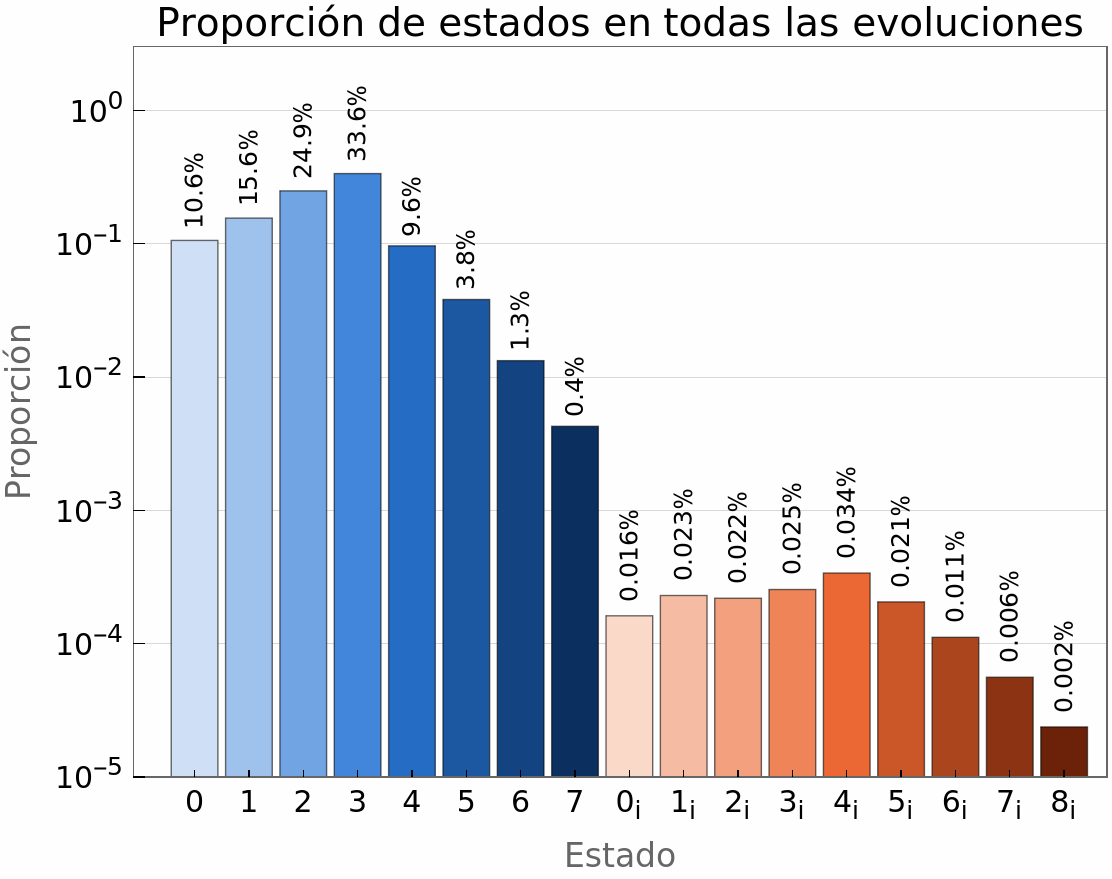
\includegraphics[width=0.7\linewidth]{img/sp_proportion.png}
	\caption{Distribuciones de probabilidad de los estados en la regla \textit{sandpile} con multiples condiciones iniciales aleatorias.}
	\label{fig:sp_proportion}
\end{figure}

Por otro lado, si consideramos la evolución tradicional con el espacio vació, obtenemos las proporciones de la figura \ref{fig:sp_0_porportion} donde aun existe la presencia de todos los patrones pero menos representados. 

\begin{figure}[H]
	\centering
	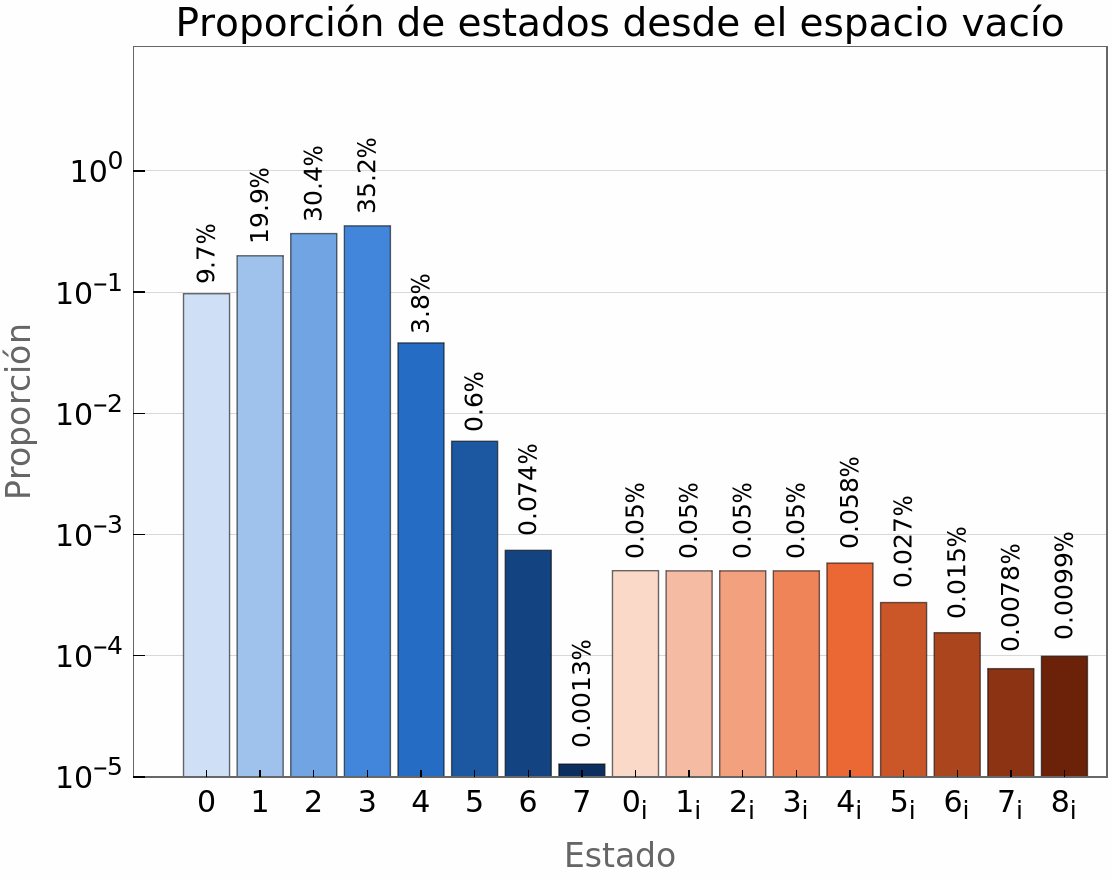
\includegraphics[width=0.7\linewidth]{img/sp_0_proportion.png}
	\caption{Distribuciones de probabilidad de los estados en la regla \textit{sandpile} con un unico generador.}
	\label{fig:sp_0_porportion}
\end{figure}

\subsubsection{Capacidad de replicación}

Como primera prueba del automata celular neuronal se utilizan las configuraciones de la tabla \ref{tab:sp_training_test}

\begin{table}[h]
	\centering
	\begin{tabular}{llrr}
		\toprule
		\textbf{Capa Oculta} & \textbf{Capa Salida} & \textbf{Épocas} & \textbf{Pérdida}\\
		\midrule
		16:16:ReLU & 17:Linear & 18 & 0.000087 \\
		16:16:TanH & 17:Linear & 35 & 0.000097 \\
		16:16:Sigmoid & 17:Linear & 79 & 0.000095 \\
		\bottomrule
	\end{tabular}
	\caption{Comparativa de rendimiento con múltiples hiperparámetros de la regla B3/S23: Pérdida objetivo 0.0001, límite de épocas: 1000, 
		tamaño del lote: 8192, tasa de aprendizaje: 0.001, semilla aleatoria: 42.}
	\label{tab:sp_training_test}
\end{table}





